\section{Performance}
\label{sec:performance}

\subsection{Component Performance}
\label{sec:performance_components}

Note: Where in the program is time spent? How much time does each thing take? (BigInteger conversion is probably
a time-stealer!!!)

Note: Introduction to performance using the Visual Studio Profiling Tools. Appendix with raw data.

\begin{figure}[htb]
	\centering
	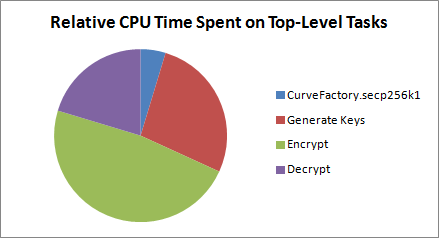
\includegraphics[width=0.70\textwidth]{performance/top-level--relative-time}
\end{figure}

Note: Introduce areas that will be investigated. Also mention that encryption is the heaviest load (above, introductory graph). Mention
that a negligible amount of time is spent encoding and decoding (compared to encryption and decryption) -- no graph needed.

\subsubsection{Point Multiplication}
\label{sec:performance_components_multiplication}

\begin{figure}[htb]
	\centering
	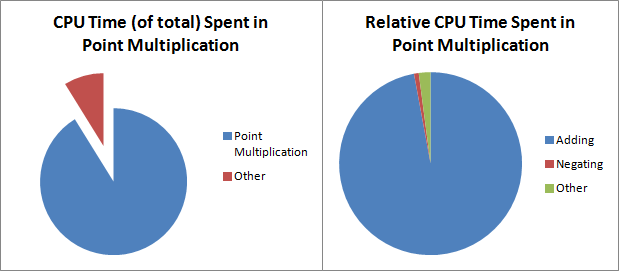
\includegraphics[width=1\textwidth]{performance/point-multiplication--relative-time}
\end{figure}

\subsubsection{Finite Field Operations}
\label{sec:performance_components_finitefield}

\begin{figure}[htb]
	\centering
	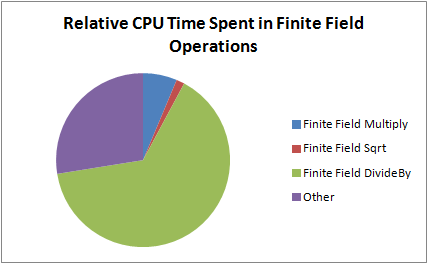
\includegraphics[width=0.6\textwidth]{performance/finite-field--relative-time}
\end{figure}

\subsubsection{BigInteger Conversion}
\label{sec:performance_components_biginteger}

\begin{figure}[htb]
	\centering
	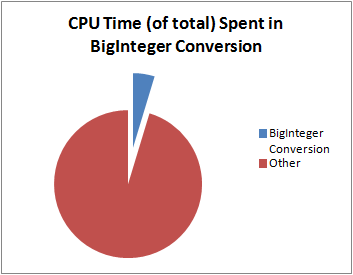
\includegraphics[width=0.6\textwidth]{performance/biginteger-conversion--relative-time}
\end{figure}

\subsection{BouncyCastle Comparison}
\label{sec:performance_bouncycastle}
Note: Measure against bouncycastle encryption with the same curve. Create beautiful (but devastating) graph!